\chapter{Aplicación}

\section{Comportamiento de Aplicación}
El punto de vista Comportamiento de la aplicación describe el comportamiento interno de una aplicación; Por ejemplo, ya que realiza uno o más servicios de aplicación. Este punto de vista es útil para diseñar el comportamiento principal de las aplicaciones o para identificar la superposición funcional entre diferentes aplicaciones.
\subsection{Modelo}
\begin{figure}[h!]
	\centering
	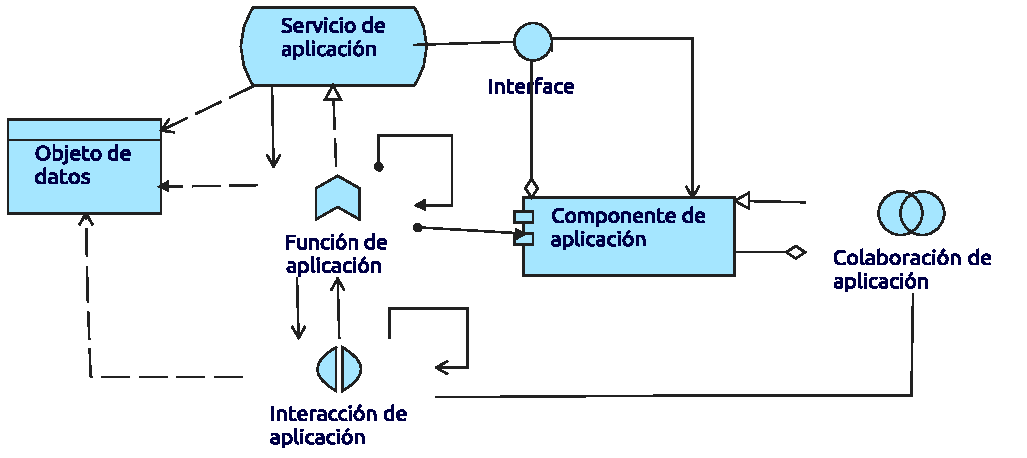
\includegraphics[width=\linewidth]{Arquitectura/Aplicacion/imgs/ComportamientoMetamodelo.pdf}
	\caption{Organización}
\end{figure}
\newpage
\subsection{Caso de Estudio}

\begin{figure}[h!]
	\centering
	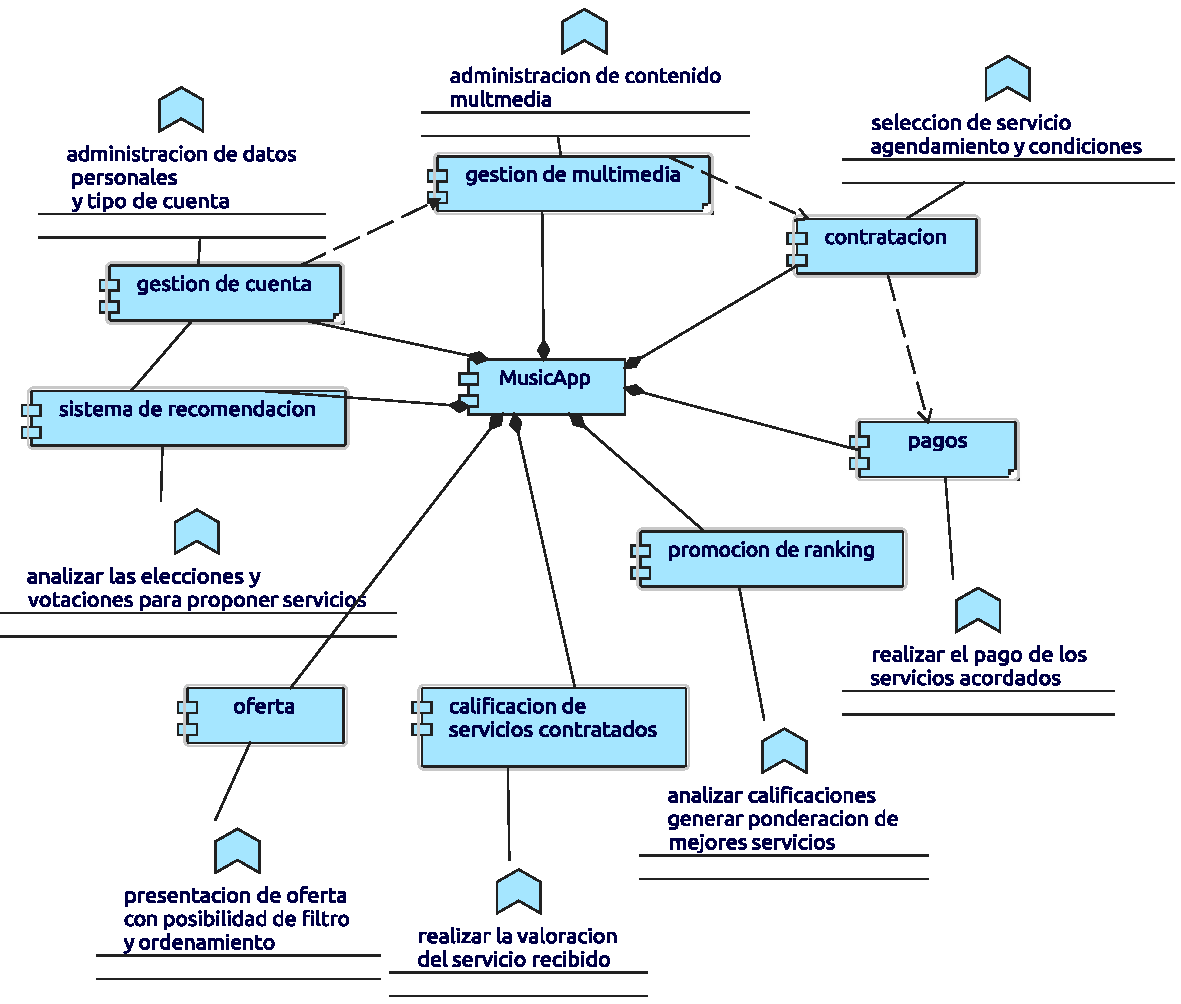
\includegraphics[width=\linewidth]{Arquitectura/Aplicacion/imgs/Comportamiento.pdf}
	\caption{Caso}
\end{figure}

\newpage

\section{Cooperación de Aplicación}
El punto de vista de la Cooperación en la Aplicación describe las relaciones entre los componentes de las aplicaciones en términos de los flujos de información entre ellos, o en términos de los servicios que ofrecen y utilizan. Este punto de vista se suele utilizar para crear una visión general del panorama de aplicaciones de una organización. Este punto de vista también se utiliza para expresar la cooperación (interna) u orquestación de servicios que en conjunto apoyan la ejecución de un proceso de negocios.
\subsection{Modelo}
\begin{figure}[h!]
	\centering
	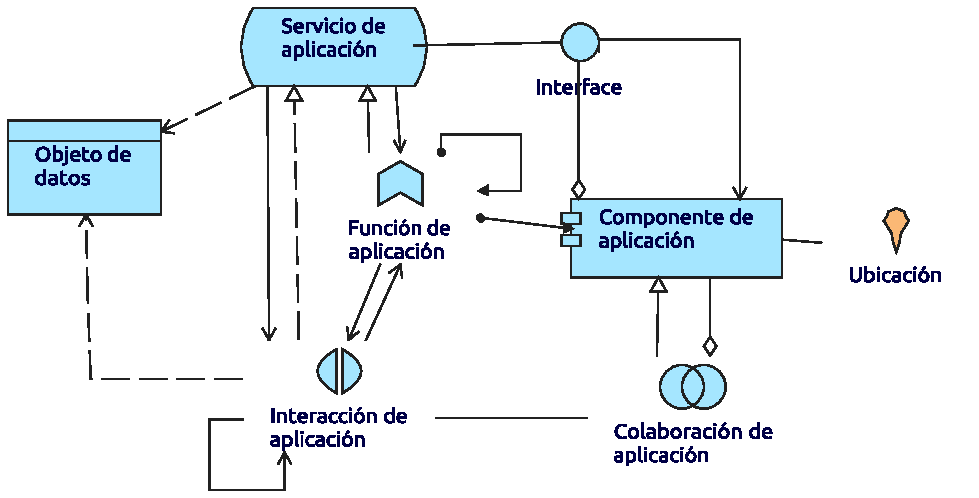
\includegraphics[width=\linewidth]{Arquitectura/Aplicacion/imgs/CooperacionMetamodelo.pdf}
	\caption{Organización}
\end{figure}
\newpage
\subsection{Caso de Estudio}

\begin{figure}[h!]
	\centering
	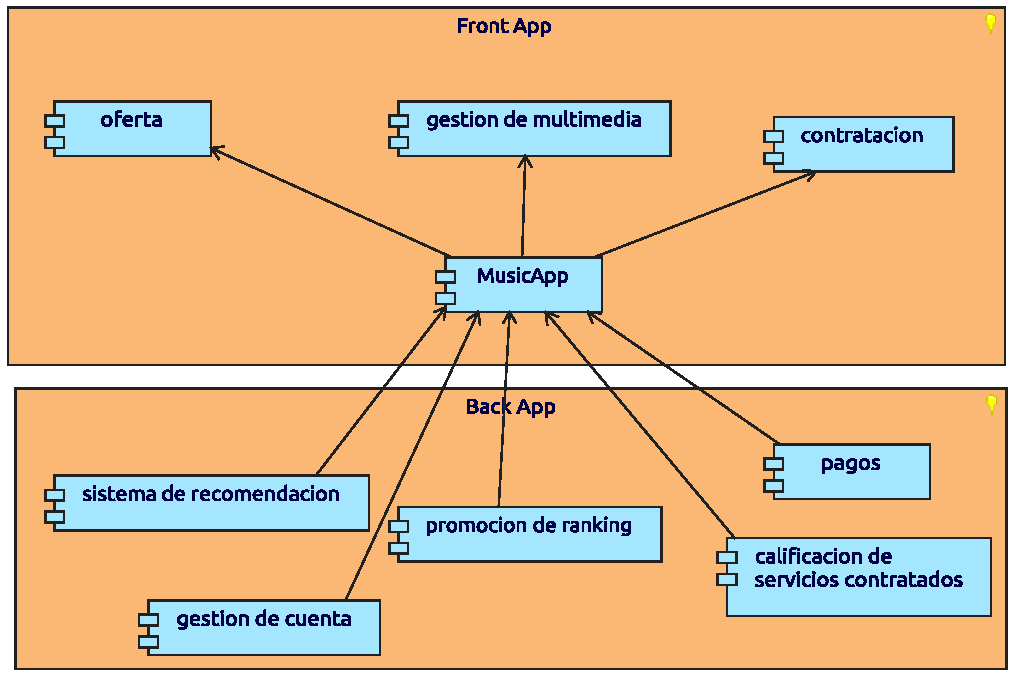
\includegraphics[width=\linewidth]{Arquitectura/Aplicacion/imgs/Cooperacion.pdf}
	\caption{Caso}
\end{figure}

\newpage